\documentclass{tufte-handout}

\usepackage{amsmath}  % extended mathematics
\usepackage{amsfonts}
\usepackage{amsthm}
\usepackage{amssymb}
\usepackage{amsfonts}
\usepackage{amsthm}

\usepackage{framed}
\usepackage{graphicx}
\usepackage{fancyhdr}

\pagestyle{fancy}
\lhead{DS100}
\chead{} 
\rhead{}

\renewcommand{\P}[0]{\mathbb{P}}
\newcommand{\E}[0]{\mathbb{E}}
\DeclareMathOperator{\Var}{Var}
\DeclareMathOperator{\SD}{SD}
\newenvironment{note}{
%  \medskip
  \begin{framed}
    \bgroup\color{black}
    {\textbf{Note}}
}{
\egroup\end{framed}
%  \medskip
}

\newcommand{\twolines}[0]{\quad \par \quad \par}

\title{DS100: Probability}
\author{Prof. Deborah Nolan}
\date{\marginnote{Scribe: Simon Mo}}


\begin{document}
\maketitle
%\tableofcontents

Recall that a simple random sample draws units from a population without replacement and at each draw all units remaining are equally likely to be selected. When we sample with replacement, at each draw all units in the population are available.

Today we will examine the distribution of random outcome. We will define expected value, variance, and standard deviation of random outcome. We will also examine the distribution of the average. 

We start with a small population to help make the core idea more transparent. 

\begin{center}
	Population: $5$ restaurants\\
	Outcome: scores $[80,80,92,92,96]$
\end{center}

With a population we can examine its distribution visually and compute summaries of the values, which are referred to as parameters. We can draw the histogram\footnote{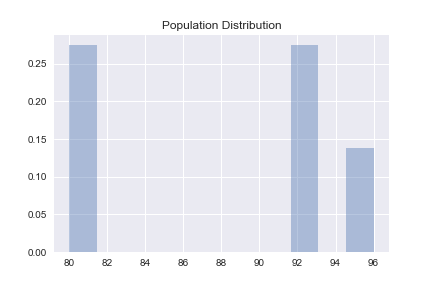
\includegraphics[width=6cm]{dist}} or compute the probability in a distribution table:\begin{center}
	\begin{tabular}{l|ccc}
  values & $80$& $92$ & $96$\\
  \hline
  prop of pop & $\frac{2}{5}$ &$\frac{2}{5}$&$\frac{1}{5}$ \\
\end{tabular}
\end{center}

We now calculate the population average and variance: \begin{align*}
	\theta^* &= (80+80+92+92+96)/5 \\
					&= 80 \times \frac{2}{5} + 92 \times \frac{2}{5} + 96 \times \frac{1}{5} \\
					&= 88 \\
	\sigma^2 &= (80-88)^2 \times \frac{2}{5} +(92-88)^2 \times \frac{2}{5} +(96-88)^2 \times \frac{1}{5} \\
				&= 64 \times \frac{2}{5} +16\times \frac{2}{5} +64 \times \frac{1}{5} \\
				& \approx 44 \end{align*}

Now think of the chance process: draw a restaurant at random and record the inspection score. We denote $X$ as the result of this chance process. What is the change the draw resulted in $80$? We express this as\marginnote{\twolines $\P$ is the probability. $X$ is the chance percent. There are two possible outcomes of the 5 restaurants. Since they are equally likely, the chance is $\frac{2}{5}$}\begin{equation*}
	\P(x=80) = \frac{2}{5}
\end{equation*}

The probability distribution table. Notice this table looks like the population distribution table. Why? Because each restaurant is \emph{equally likely}.
\begin{center}
	\begin{tabular}{l|ccc}
  values & $80$& $92$ & $96$\\
  \hline
  chance & $\frac{2}{5}$ &$\frac{2}{5}$&$\frac{1}{5}$ \\
\end{tabular}
\end{center}

\section{Expected Value}
\begin{align*}
	\E(X) &= 80\P(X=80) + 92\P(X+92) + 96\P(X=96) \\
	&= 80 \times\frac{2}{5} + 92 \times\frac{2}{5} + 96 \times\frac{1}{5} \\
	&= 89 \\
	&= \theta^*
\end{align*}
The expected value of $X$ matches the population parameter (mean).

\section{Variance}
\begin{align*}
	\E(X-\E(X))^2 &= \E(X-\theta^*)^2 \\
	&= (80 - \theta^*)^2\P(X=80)  +  (92 - \theta^*)^2\P(X=92)  +  (96 - \theta^*)^2\P(X=96)  \\
	&=\sigma^2
\end{align*}
We can substitute 88 for $\theta^*$ and calculate the probability to get the value. 

\section{Generalize}
Suppose we have a random variable $X$ with the probability distribution \marginnote{$v_j$ is the values that $x$ could take on. $p_j$ is the chance, it is between $0$ and $1$} \begin{equation*}
	\P(X = v_j) = P_j \quad \quad j= 1, \ldots, m
\end{equation*}

We have \begin{align*}
	\E(X) &= \sum_{j=1}^m v_j p_j \quad i.e. v_j\P(X=v_j) \\
	\Var(X) &= \E (X-\E(X))^2 \\
		           &= \sum_{j=1}^m (v_j - \E(X))^2 p_j\\
	\SD(X) &= \sqrt{\Var(X)}\\
\end{align*}

\paragraph{Some useful properties of expectation} 

Suppose the transform $X$ linearly, $Y=aX+b$.

Find $\E(Y), \Var(Y) \SD(Y)$ in terms of $\E(X), \Var(X), \SD(X)$

\begin{align*}
	\E(Y) &= \sum_{j=1}^m y_j \P(Y=y_j) && y_j = av_j + b \\
	&= \sum_{j=1}^m (av_j + b) p_j \\
	&= \sum_{j=1}^m (av_j p_j + bp_j)  && a,b \text{ do not depend on } j \\
	&= a\sum_{j=1}^m v_jp_j + b \sum_{j=1}^m p_j && \sum_{j=1}^mp_j = 1 \\
	&= a\E(x) + b  \\
	\Var(Y) &= \E(Y-\E(Y))^2 \\
	&= \E(aX+b-(a\E(X)+b))^2 && \text{ from above} \\
	&= a^2 \E(X-\E(X))^2 \\
	&= a^2 \Var(x) \\
	\SD(Y) &= |a| \SD(X)
\end{align*}

The second draw. Now let $X_2$ be the result of the second draw from our population. For now, let's assume the draws are \emph{with} replacement. 

What is $X_2$'s distribution? Expected value, Variance, SD? 

We start with its probability distribution. Since all elements are still available to be drawn, the probability of $X_2$ is the same as $X_1$ (we relabel $X$ as $X_1$)
\begin{center}
		\begin{tabular}{l|ccc}
  $X_2$ values & $80$& $92$ & $96$\\
  \hline
  chance & $\frac{2}{5}$ &$\frac{2}{5}$&$\frac{1}{5}$ \\
\end{tabular}
\end{center}

Since the distribution are the same, the expected value, variance, and $\SD$ will be the same. \begin{equation*}
	\E(X_2) = \E(X_1) = 88 \quad \quad \Var(X_2) = \Var(X_1)
\end{equation*}

Next, we consider the average $\bar{X} = \frac{X_1 + X_2}{2}$. Note this is a random variable too. Sometimes the average is $80$, when both draws are $80$ or $86$ when one draw is $80$ and the other is $92$. What are teh values $\bar{X}$ can take on? \marginnote{\twolines Where dose the chance, say $\frac{8}{25}$ comes from? The denominator is $25$ because there are $5 \times 5 =25$ possible pairs $(X_1,X_2)$, $8$ of these $25$ have an average of $86$. These are $
	(80_a, 92_a), (80_a, 92_b), (80_b, 92_a)$, $(80_b, 92_b), (92_a, 80_a), (92_a, 80_b) $, $(92_b, 80_a), (92_b, 80_b)$\\ Note we put subscript $\ _a,\ _b$ on the value to distinguish them. }
\begin{center}
		\begin{tabular}{l|cccccc}
  $\bar{X}$ values & $80$& $86$ & $88$ &$92$ & $94$ & $96$\\
  \hline
  chance & $\frac{4}{25}$ & $\frac{8}{25}$ & $\frac{4}{25}$&$\frac{4}{25}$ & $\frac{4}{25}$ & $\frac{1}{25}$ \\
\end{tabular}
\end{center}
This is the probability distribution table for $\bar X$.

What about $\E(\bar X)$?
\begin{align*}
	\E(\bar X) &= \E (\frac{1}{2} (X_1+X_2)) \\
	&= \frac{1}{2} \E (X_1+X_2) && \text{by linearity} 
\end{align*}
Now we need to find $\E(X_1 + X_2)$. From the general definition: \begin{equation*}
	\E(X_1 + X_2) = \sum_{j=1}^m\sum_{k=1}^m (v_j + v_k) \P(X_1 = v_j, X_2 = v_k)
\end{equation*}

How do we proceed? We need to understand how random variable can vary together. 

\section{Aside: Joint Distribution}
$\P(X_1 = v_j, X_2 = v_k) = $ chance that $X_1$ is $v_j$ and $X_2$ is $v_k$. With two random variable we have joint probability: 


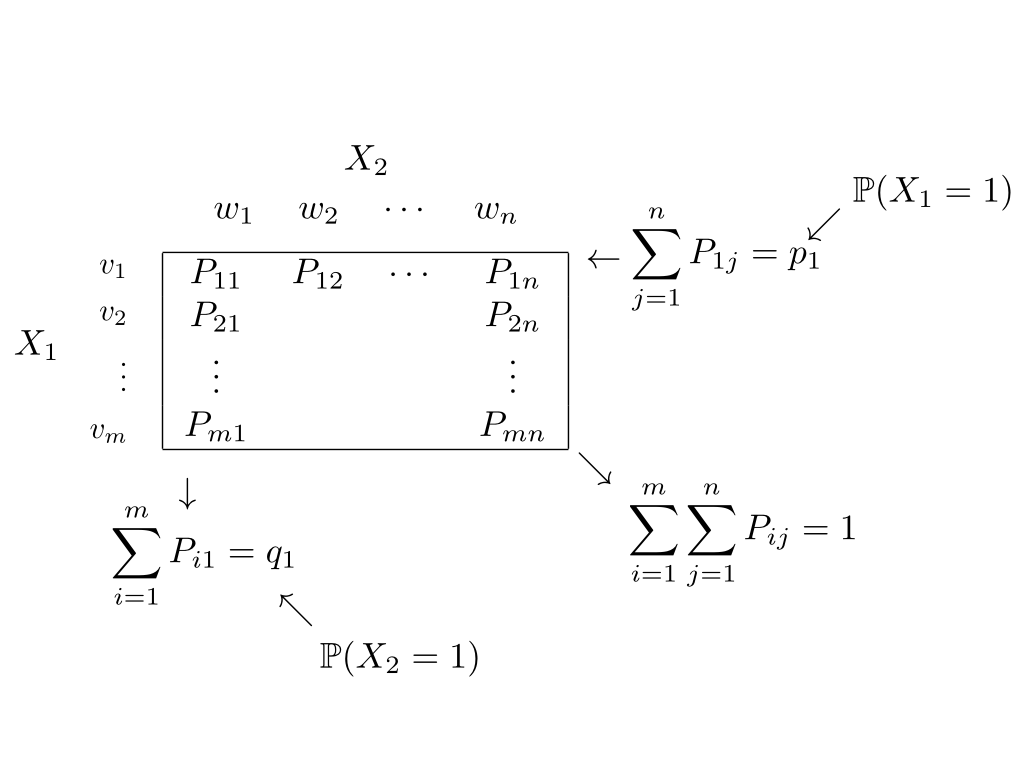
\includegraphics[scale=0.3]{joint.png}\\

Also we can  define conditional probability: $\P(X_1 = v_i, X_2 = w_j) = \P(X_1 = v_i)\P(X_2 = w_j | X_1 = v_i)$. \marginnote{\twolines $|$ means given. Note that $\sum_j \P(X_2 = w_j|X_1 = v_i) = 1$.} 

Two variables are independent when $\P(X_2 = w_j|X_1 = v_i) = \P(X_2 = w_j)$. The chance a variable takes on a value does not change given the knowledge that the second variable has a particular value. 

Let's return to computing $(X_1 + X_2)$'s expected value.
\begin{align*}
	\E(X_1 + X_2) &= \sum_{j=1}^m\sum_{k=1}^m (v_j + v_k) \P(X_1 = v_j, X_2 = v_k)\\
	&= \sum_{j=1}^m v_j \sum_{k=1}^m \P(X_1 = v_j, X_2 = v_k) +  \sum_{k=1}^m v_k \sum_{j=1}^m  \P(X_1 = v_j, X_2 = v_k) \\
	&= \sum_{j=1}^m v_j \P(X_1 = v_j) + \sum_{k=1}^m  v_k \P(X_2 = v_k) \\
	&= \E(X_1) + \E(X_2)
\end{align*}
Notice that we did not use independence to derive above. This means: \begin{equation*}
	\E(\bar X) = \frac{1}{2} \E(X_1 + X_2) = \frac{1}{2} [\E(X_1) + \E(X_2)] = \theta^*
\end{equation*}

What about $\Var(\bar X)$?

\begin{align*}
	\Var(\bar X) &= \E(\bar X - \theta^*)^2 \\
	&= \E(\frac{1}{2} \sum_{i=1}^2 X_i - \theta^*)^2 \\
	&= \E(\frac{1}{2} \sum_{i=1}^2 (X_i - \theta^*))^2 \\
	&= \frac{1}{4} \E[(X_1 - \theta^*)^2 + (X_2 - \theta^*)^2 + 2(X_1 - \theta^*)(X_2 - \theta^*)] \\
	&= \frac{1}{4} [\Var(X_1) + \Var(X_2) + 2\E (X_1 - \theta^*)(X_2 - \theta^*) \\
	&= \frac{\sigma^2}{2} + \frac{1}{2}\E (X_1 - \theta^*)(X_2 - \theta^*)
\end{align*}

We can use the result that for independent random variables $\E(XY) = \E(X)\E(Y)$. \marginnote{can you prove this?}
Note also $\E(X_1 - \theta^*) = \E(X_1) - \theta^* = \theta^* - \theta^* = 0$. All together, this leads to: \begin{equation*}
	\Var(\bar X) = \frac{\sigma^2}{2} \text{ and } \SD(\bar X) = \frac{\sigma}{\sqrt{2}}
\end{equation*}

In general, for independent random variables, \begin{equation*}
	\Var(\bar X) = \frac{\sigma^2}{n} \text{ and } \SD(\bar X) = \frac{\sigma}{\sqrt{n}}
\end{equation*}

Finally, let's consider the case where we draw from the population without replacement, i.e., SRS. In our sample population: $80,80,92,92,96$. We have:\begin{center}
	$X_1 = $ result of first draw \\
	$X_2 = $ result of second draw \\
\end{center}
We knwo the probability distribution for $X_1$ is   	\begin{tabular}{l|ccc}
  values & $80$& $92$ & $96$\\
  \hline
  chance & $\frac{2}{5}$ &$\frac{2}{5}$&$\frac{1}{5}$ \\
\end{tabular}

Are $X_1$ and $X_2$ independent? No.

Because \begin{equation*}
	\P(X_2 = 96) = \frac{1}{5} \text{ but } \P(X_2 = 96 | X_1 = 96) = 0
\end{equation*}
So the probability changes if we know $X_1$'s value. The joint probability distribution of $(X_1, X_2)$ for our SRS:

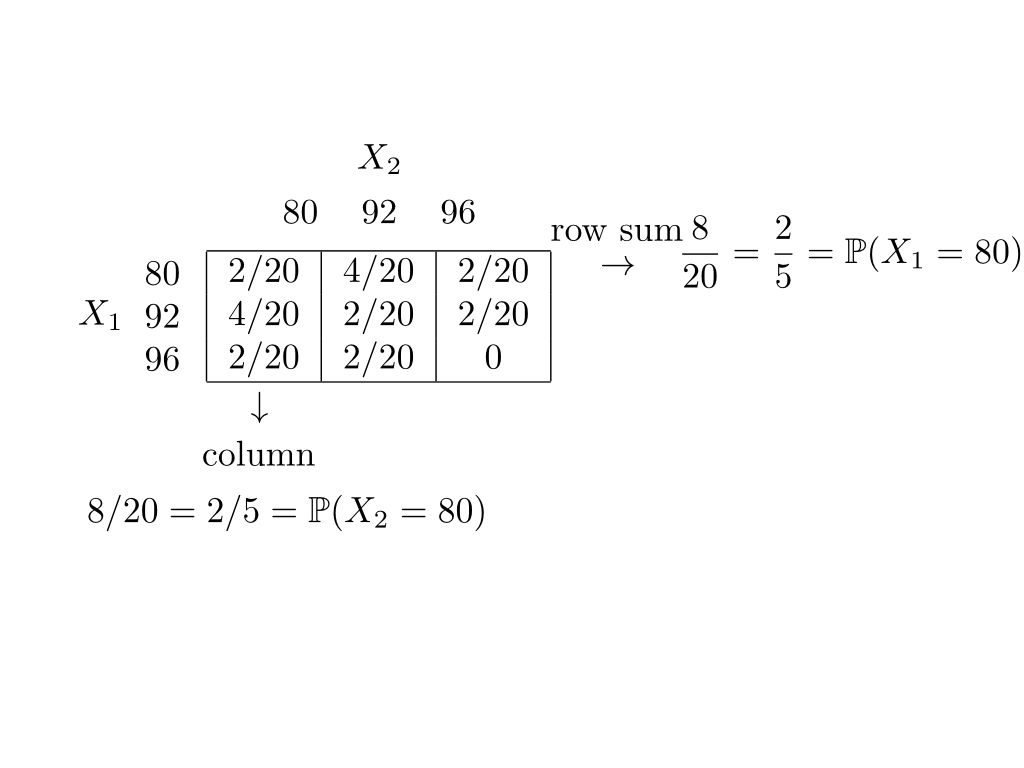
\includegraphics[scale=0.3]{joint2.png}\\
Recall that in our proof that $\E(\bar X) = \theta^*$\footnote{$88$ in this case}. We only used the row and column sums of the table. We did not use independence. This means:\begin{center}
	$\E(\bar X) = \theta^*$ for sampling with out replacement.
\end{center}
However when we compute $\Var(\bar X)$ we used independence to find $\E(X_1 - \theta^*) (X_2 - \theta^*)  = 0$. IN the dependent case, this is not so. We will not prove this result. For a SRS of $n$ units from a population of $N$. \begin{equation*}
	\Var(\bar X) = \frac{N-n}{N-1}\frac{\sigma^2}{n}
\end{equation*}
$\frac{N-n}{N-1}$ accounts for the dependent. It says that $\bar X$ is less variable when we don't replace units between draws. \marginnote{What is $\Var(\bar X)$ when $n=N$? Does this make sense?}
\end{document}